\section{ZIOTP2026: A Dataset for Zigbee traffic classification}
\label{ZIOTP2026}
Despite the widespread adoption of Zigbee in smart home environments, publicly available Zigbee traffic datasets remain scarce. To address this gap and support reproducible research, we introduce ZIOTP2026, a dataset of Zigbee network traffic collected over multiple days in realistic smart home settings and capturing natural user-device interactions. The data collection methodology builds upon prior work \cite{iot_dataset_paper}, extending its Zigbee component by capturing traffic from 21 off-the-shelf devices spanning 15 models and seven manufacturers.
To enable the investigation of topology-dependent effects, devices were deployed across two distinct Zigbee personal area networks (PANs) during data acquisition. This multi-topology design allows systematic analysis of how network configuration impacts traffic-based forensic tasks such as device classification and identification.


\subsection{Acquisition Setup}
\label{Data_acquisition_Setup}
A dedicated network architecture was deployed to replicate a realistic smart home environment. An isolated \gls*{lan} was configured using a consumer-grade router running OpenWRT, with a Raspberry Pi running Home Assistant OS \cite{home_assistant_os} acting as the central smart home gateway and Zigbee \gls*{panc}. Zigbee connectivity was provided through a USB radio interface managed by the \gls*{zha} integration\footnote{https://www.home-assistant.io/integrations/zha/}, which handled network formation and device onboarding. For all experiments, the \gls*{pan} was configured on Channel~11 and devices were added in isolation to ensure reproducible initialization.

IP-based traffic exchanged within the \gls*{lan} was captured from a host connected to the network, which also provided access to the Home Assistant dashboard. Zigbee traffic at the IEEE~802.15.4 layer was collected using a dedicated packet sniffer operating in promiscuous mode. To ensure reliable capture, the sniffer and the Zigbee radio interface were placed in close proximity. The overall network configuration is illustrated in Figure~\ref{fig:Chapter4:network_configuration}.

To analyze the impact of network topology on Zigbee traffic analysis, data acquisition was conducted under two distinct Zigbee network topologies. Here, topology refers to the spatial arrangement of devices and the resulting communication paths among the \gls*{panc}, \glspl*{ffd}, and \glspl*{redfd}. Unlike Wi-Fi’s star topology, Zigbee relies on mesh communication, where messages may be forwarded through intermediate \glspl*{ffd}. The two adopted topologies, shown in Figure~\ref{fig:Chapter4:device_topology}, differ in device placement and coordinator position, inducing distinct multi-hop communication patterns. The acquisition procedure was kept identical across both topologies.

\begin{comment}
\subsection{Acquisition Setup}
\label{Data_acquisition_Setup}
A dedicated network architecture was deployed to replicate a realistic smart home environment. A GL.iNet GL-AR300M16-Ext router running OpenWRT was used to create an isolated \gls*{lan}, emulating typical residential smart home networking conditions. Within this \gls*{lan}, a Raspberry Pi 4 Model B running Home Assistant OS \cite{home_assistant_os} acted as the central smart home gateway. Zigbee connectivity was provided by a Sonoff EFR32MG21 USB module, which operated as the \gls*{panc} and served as the radio interface for Zigbee communications.

The Zigbee \gls*{pan} was created and managed through the \gls*{zha} integration\footnote{https://www.home-assistant.io/integrations/zha/}
 available in Home Assistant OS. This integration automatically interfaced with the Sonoff EFR32MG21 dongle \cite{efr32_dongle} connected to the Raspberry Pi, enabling network formation and device onboarding. For all experiments, the \gls*{pan} was configured on Channel~11, and devices were added in isolation to ensure controlled and reproducible network initialization.

A laptop connected to the same \gls*{lan} was used to capture IP-based traffic traversing the GL.iNet router and to access the Home Assistant dashboard for device configuration and control. Zigbee traffic at the IEEE~802.15.4 layer was captured using a Texas Instruments CC2531 USB dongle \cite{ti_cc2531_datasheet}. The CC2531 is an IEEE~802.15.4-compliant wireless transceiver equipped with a dedicated packet sniffer firmware\footnote{https://www.ti.com/tool/PACKET-SNIFFER}
, enabling promiscuous-mode traffic capture. The dongle was connected to the laptop, and Zigbee traffic was collected using the \textit{whsniff} tool \cite{whsniff}. To maximize capture reliability, the Zigbee sniffer and the Zigbee radio interface connected to the Raspberry Pi were placed in close proximity (less than 5~cm apart). The overall network configuration is illustrated in Figure~\ref{fig:Chapter4:network_configuration}.

To investigate the impact of network topology on Zigbee traffic analysis, data acquisition was conducted across two distinct Zigbee network topologies. Here, topology refers to the spatial disposition of IoT devices within the smart home environment and the resulting communication paths among the \gls*{panc}, \glspl*{ffd}, and \glspl*{redfd}. Unlike Wi-Fi networks, which typically follow a star topology with direct client-to-access-point communication, Zigbee networks rely on mesh topologies, where messages may be forwarded through intermediate \glspl*{ffd} acting as relays.

The two topologies adopted in the acquisition campaign are shown in Figure~\ref{fig:Chapter4:device_topology}. In each topology, both the placement of devices and the position of the \gls*{panc} were varied to induce different multi-hop communication patterns. In the figure, colors are used to distinguish the mesh networks formed between \glspl*{redfd} and their associated \glspl*{ffd}, while devices shown in white are directly connected to the \gls*{panc}. These configurations were designed to assess whether changes in network topology affect device identification and classification performance, given that Zigbee’s mesh routing behavior and the underlying IEEE~802.15.4 physical layer can significantly influence observable traffic features. The data acquisition procedure was kept identical across the two topologies and is described in detail in the following section.
\end{comment}

\begin{figure}[t]
    \centering
    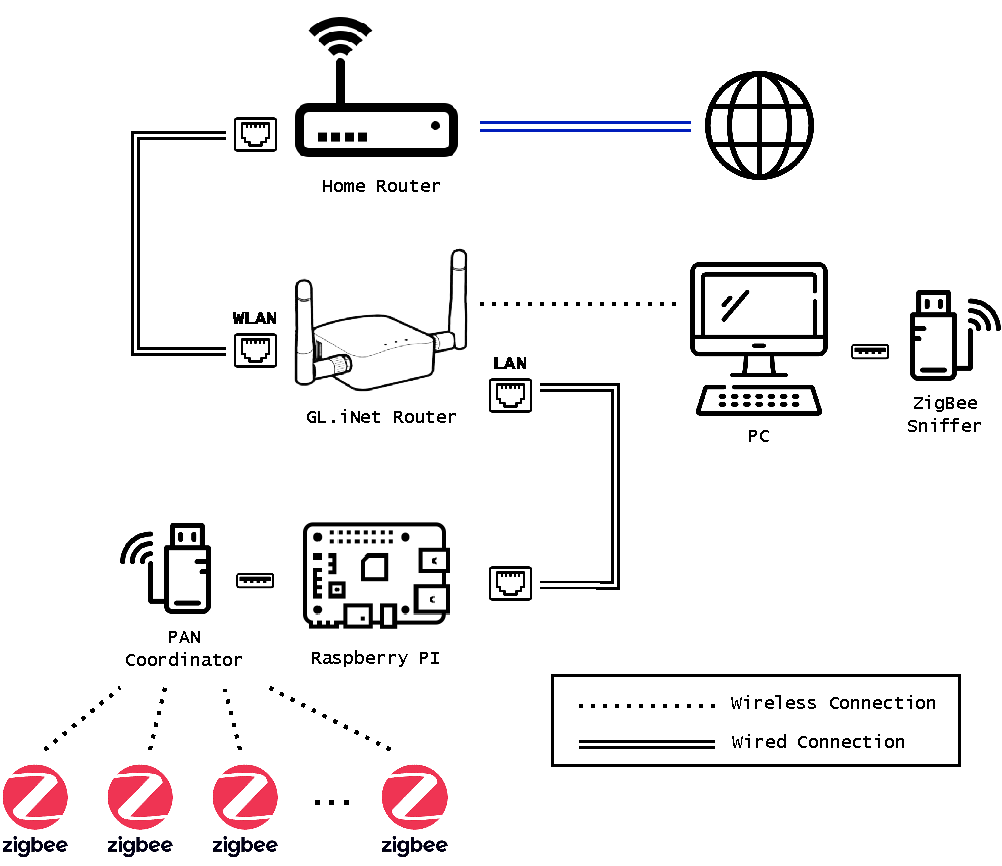
\includegraphics[width=0.65\columnwidth]{Figures/Network_Configuration.pdf}
    %\caption{Network configuration of the smart home and the acquisition pipeline for capturing ZigBee-based network traffic from commercial IoT devices. The smart home is controlled by a Raspberry Pi 4 and by a PAN coordinator (based on the EFR32MG21 SoC). The acquisition setup is represented by a Laptop and a Zigbee Sniffer (based on CC2531 SoC), which aims to capture IP and ZigBee-based network traces. An extra mini Router has been added to the Smart Home network to isolate the network.}
    \caption{Network configuration of the smart home and acquisition pipeline used to capture Zigbee and IP traffic from commercial IoT devices. The smart home is managed by a central gateway acting as PAN coordinator, while a dedicated sniffer and a monitoring host capture Zigbee and IP network traces within an isolated network.}
    \label{fig:Chapter4:network_configuration}
\end{figure}

\begin{figure}[t]
    \centering

    \begin{subfigure}[b]{0.4\textwidth}
        \centering
        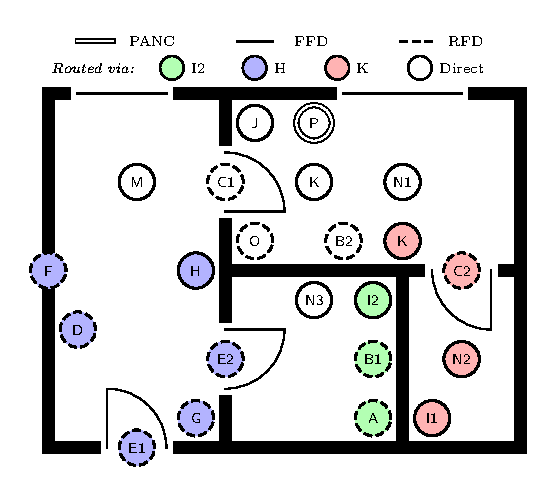
\includegraphics[width=\textwidth,trim={10 14 10 15},clip]{Figures/connection_structure/topA.pdf}
        \caption{Topology A}
        \label{fig:subfig1_A}
    \end{subfigure}
    \hfill
    \begin{subfigure}[b]{0.39\textwidth}
        \centering
        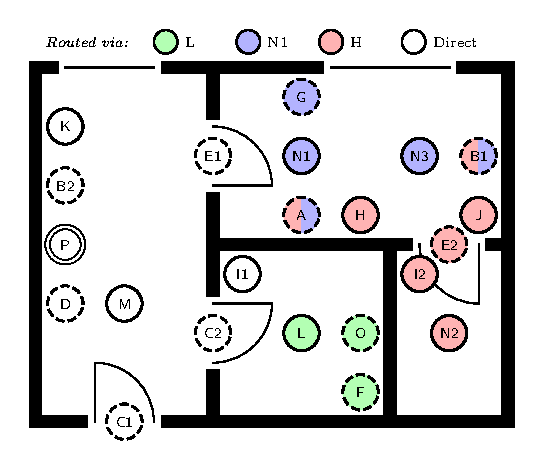
\includegraphics[width=\textwidth,trim={10 14 10 14},clip]{Figures/connection_structure/topB.pdf}
        \caption{Topology B}
        \label{fig:subfig2_B}
    \end{subfigure}
\caption{Device disposition during the acquisition campaign for the two considered topologies.
Devices are positioned according to their physical deployment and labeled as reported in Table \ref{tab:dataset}.
The outer line style identifies the device role (PANC, FFD, or RFD).
Color coding indicates the logical communication path toward the PANC: white denotes devices directly associated with the PANC, while colored devices communicate with the PANC via an intermediate FFD acting as a router.} 
\label{fig:Chapter4:device_topology} 
\end{figure}

\subsection{Acquiring Device Behaviors}
\label{acq_behav}
Following the acquisition methodology introduced in \cite{iot_dataset_paper}, a set of controlled interaction scenarios was designed to capture a wide range of Zigbee device behaviors and operational states. The acquisition campaign included: (i) idle periods with no user interaction, used to characterize background and periodic traffic; (ii) power cycling events for mains-powered devices, capturing network join and leave procedures; (iii) user-issued commands executed through the smart home controller; (iv) direct physical interactions with sensors (e.g., motion, door, vibration); and (v) extended active scenarios emulating natural day-to-day smart home usage. Each scenario was repeated multiple times to capture temporal variability and enrich the dataset with diverse traffic patterns.

\subsection{Ground Truth Extraction}
Since the dataset captures encrypted Zigbee traffic, device identity and application-layer payloads are not directly observable. Device identities were recovered a posteriori by isolating each device and associating its traffic with the corresponding IEEE MAC address. To enable event-level labeling, each device was individually reset and paired with the \gls*{panc}, while Zigbee traffic exchanged during the pairing phase was captured.

During commissioning, the transport key is exchanged within the Zigbee Application Support (APS) layer and encrypted using a publicly known trust center link key. Leveraging this mechanism, pairing traffic was decrypted using Wireshark\footnote{https://www.wireshark.org/} to extract the device-specific transport key, which was then used exclusively for dataset labeling and validation.

All subsequent traffic analysis and machine learning experiments were performed on encrypted traffic only, without relying on decrypted payload information.


\begin{comment}
\subsection{Acquiring Device Behaviors}
\label{acq_behav}
Following the data acquisition methodology introduced in \cite{iot_dataset_paper}, a set of controlled experiments was conducted to enrich the dataset with a wide range of IoT device behaviors and operational states. 

\subsubsection{Idle Phase}
During the Idle Phase, the smart home environment was left inactive for one hour, with no user-initiated interactions. The objective of this phase was to capture baseline Zigbee traffic generated solely by periodic device communications and internal protocol operations. This traffic provides a reference representation of network behavior in a quiescent state, enabling the characterization of background communication patterns. The Idle Phase was repeated three times to account for temporal variability.

\subsubsection{Power Cycling Phase}
The Power Cycling Phase aimed to capture Zigbee traffic associated with device join and leave events. For each non-battery-powered device, a controlled routine was executed in which the device was disconnected from power, reconnected for two minutes, and then disconnected again for three minutes. This sequence was repeated three times per device, allowing the collection of traffic traces related to network re-association, initialization, and teardown procedures.

\subsubsection{Command Interaction Phase}
The Command Interaction Phase focused on capturing Zigbee traffic generated by explicit user commands issued through the Home Assistant web interface and smartphone application connected to the isolated \gls*{lan}. Typical commands included device activation, deactivation, and state changes. In parallel, IP-based traffic exchanged between the user interfaces and the smart home gateway was captured using TCP dump. This additional capture enables the investigation of potential correlations between IP-layer interactions and Zigbee frame-level activity.

\subsubsection{Physical Interaction Phase}
In the Physical Interaction Phase, Zigbee traffic was collected in response to direct human interactions with devices, such as walking near motion sensors, pressing physical buttons, opening doors, or inducing vibrations. The goal of this phase was to capture communication patterns generated by sensor-triggered events that occur independently of centralized control applications.

\subsubsection{Active Interaction Phase}
The Active Interaction Phase was designed to emulate a realistic household environment by capturing Zigbee traffic during natural day-to-day activities. This scenario included a mixture of user commands, sensor activations, and routine events occurring over time, thereby reflecting typical smart home operation under normal usage conditions.

\subsection{Ground Truth Extraction}
Since the dataset is designed to capture encrypted Zigbee traffic, some information is not directly observable from packet contents. In particular, two key elements are not accessible in plaintext: the device identity (i.e., device name and type) and the application-layer payload. While device identity can be recovered a posteriori by isolating each device and associating its observed traffic with its unique IEEE MAC address, payload information remains encrypted throughout normal network operation.

In Zigbee networks, application payloads are protected using symmetric encryption, where each device shares a unique network or link key with the \gls*{panc}. This key is generated during the pairing process and subsequently used to encrypt end-to-end communications. To enable ground truth extraction, each device was individually reset and placed in pairing mode to initiate a new association with the \gls*{pan} Coordinator on the \gls*{pan} described in Section~\ref{Data_acquisition_Setup}. During this process, the CC2531 sniffer was used to capture all Zigbee traffic exchanged between the device and the coordinator.

Capturing the initial pairing phase enables the recovery of the transport key exchanged during device commissioning. Specifically, the transport key is conveyed within the Zigbee Application Support (APS) layer and is itself encrypted using a default, publicly known AES-128 trust center link key. By leveraging this well-known key, it is possible to decrypt the pairing traffic and extract the newly generated transport key associated with the device.

Traffic decryption and key extraction were performed using Wireshark\footnote{https://www.wireshark.org/}, which supports Zigbee protocol analysis and decryption when appropriate keys are provided. This procedure allowed us to decrypt Zigbee traffic solely for the purpose of dataset labeling and validation, enabling the association of observed traffic traces with device identities, device types, and interaction events.

It is important to note that the extracted transport keys were used exclusively to generate ground truth labels and to clean the dataset. All subsequent traffic analysis and machine learning experiments presented in this work are performed using encrypted traffic only, without relying on decrypted payload information.
\end{comment}

\begin{comment}
\begin{figure}
    \centering
    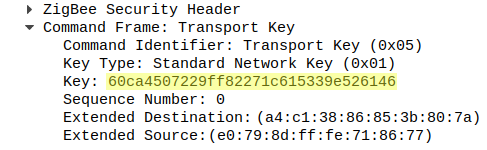
\includegraphics[width=\linewidth]{Figures/Key_Extraction.png}
    \caption{Wireshark view of a Network Transport Key extraction after decrypting the message with a pre-shared AES symmetric key }
    \label{fig:key_extraction}
\end{figure}
\end{comment}

\begin{comment}
\subsection{Dataset Characteristics and Availability}
The resulting dataset comprises a total of 252,896 IEEE~802.15.4 frames, of which 69,497 are Zigbee frames, corresponding to approximately 2,520 human-generated commands across the two considered topologies. This volume provides a representative view of Zigbee communications in a realistic smart home environment. The two topologies exhibit a nearly balanced data distribution, with Topology~B containing approximately 3\% more traffic than Topology~A.

Each topology-specific dataset has a size of approximately 17~MB and includes traffic generated by the \gls*{panc}, mains-powered devices such as smart bulbs and plugs, and battery-operated devices. In addition, around 40~MB of IP-based traffic captured during the command interaction phases is included, enabling a holistic analysis of cross-technology communication dynamics.

Although the overall dataset size may appear limited when compared to daily traffic volumes observed in IP-based networks, this characteristic is consistent with the design of Zigbee, which is optimized for the exchange of infrequent and small-sized messages. Despite its compact size, the dataset captures a broad range of device behaviors and interaction scenarios.

The dataset includes traffic from 21 distinct Zigbee-based IoT devices commercially available on the European market, covering multiple device categories such as temperature sensors, door sensors, motion detectors, smart plugs, smart bulbs, vibration sensors, and light sensors. This diversity enables the analysis of inter-manufacturer variability and device-category differentiation within a populated smart home environment. Moreover, multiple instances of selected devices are included to support comparative analyses of behavioral variability among devices of the same model and manufacturer.

Table~\ref{tab:dataset} reports the complete list of devices, along with information on model, brand, quantity, and per-device traffic contribution. The data distribution column quantifies each device’s contribution to the total volume of captured Zigbee packets. A significant imbalance in traffic volume—spanning nearly two orders of magnitude—can be observed between \glspl*{ffd} and \glspl*{redfd}, as expected given the low-power and low-duty-cycle design of battery-operated devices. This intrinsic imbalance introduces additional challenges for machine-learning-based traffic analysis, particularly in classification and identification tasks.

To foster reproducibility and encourage further research in Zigbee traffic analysis and IoT forensics, the ZIOTP2026 dataset is made publicly available.
\end{comment}
\subsection{Dataset Characteristics and Availability}
The ZIOTP2026 dataset comprises 252,896 IEEE~802.15.4 frames, including 69,497 Zigbee frames corresponding to approximately 2,520 human-generated commands collected across two network topologies. The traffic volume is nearly balanced between the two configurations, with Topology~B containing approximately 3\% more data than Topology~A. Each topology-specific dataset occupies approximately 17~MB and includes traffic generated by the \gls*{panc}, mains-powered devices (e.g., smart bulbs and plugs), and battery-operated devices. In addition, around 40~MB of IP-based traffic captured during command interaction phases is provided, enabling cross-technology analysis.
The dataset includes traffic from 21 commercial Zigbee devices spanning multiple categories (e.g., sensors, actuators, and lighting devices) and several manufacturers. Multiple instances of selected devices are included to support comparative analysis across devices of the same model. Table~\ref{tab:dataset} summarizes device models, quantities, and per-device traffic contributions. As expected, traffic volume is highly unbalanced across device roles, with \glspl*{redfd} generating up to two orders of magnitude fewer packets than \glspl*{ffd}. This imbalance reflects the low-duty-cycle design of battery-powered devices and introduces additional challenges for machine-learning-based traffic analysis.
The ZIOTP2026 dataset is publicly available to support reproducible research in Zigbee traffic analysis and IoT forensics.

\begin{table}[t]
\centering
\footnotesize
\setlength{\tabcolsep}{3pt}
\renewcommand{\arraystretch}{1.1}
\begin{tabularx}{\columnwidth}{c l X l l c c c}
\toprule
\textbf{Label} & \textbf{Brand} & \textbf{Device} & \textbf{Category} & \textbf{Model} & \textbf{Qty} & \textbf{Type} & \textbf{Data Dist.} \\
\midrule
A & Sonoff   & Temperature Sensor     & Temperature & SNZB-02       & 1 & RFD & 0.25\% \\
B & Sonoff   & Motion Sensor          & Motion      & SNZB-03       & 2 & RFD & 0.12\% \\
C & Sonoff   & Door Sensor            & Door        & SNZB-04       & 2 & RFD & 0.10\% \\
D & Aqara    & Motion Sensor P1       & Motion      & MS-S02        & 1 & RFD & 0.22\% \\
E & Aqara    & Door and Window Sensor & Door        & DW-S02D       & 2 & RFD & 0.32\% \\
F & Aqara    & Vibration Sensor       & Motion      & DJT11LM       & 1 & RFD & 0.17\% \\
G & Aqara    & Mini Switch            & Button      & WB-R02D       & 1 & RFD & 0.33\% \\
H & Tuya     & Smart Socket EU-16A    & Socket      & N/A           & 1 & FFD & 16.44\% \\
I & Senckit  & Smart Power Plug       & Socket      & N/A           & 2 & FFD & 15.38\% \\
J & Ledvance & Z3 Plug                & Socket      & 4058075208513 & 1 & FFD & 3.08\% \\
K & Ledvance & Smart+ Plug            & Socket      & 4058075729261 & 1 & FFD & 2.06\% \\
L & Ledvance & Smart+ Bulb            & Bulb        & 4058075208391 & 1 & FFD & 8.77\% \\
M & Moes     & Bulb                   & Bulb        & GU10          & 1 & FFD & 4.12\% \\
N & Philips  & HueLamp                & Bulb        & LWA019        & 3 & FFD & 5.75\% \\
O & Philips  & HueMotion              & Motion      & SML001        & 1 & RFD & 4.24\% \\
\bottomrule
\end{tabularx}
% \begin{table*}[]
% \centering
% \begin{tabular}{c c c c c c c c}
% \textbf{Label} &\textbf{Brand} & \textbf{Device} & \textbf{Category} & \textbf{Model} & \textbf{Qty} & \textbf{Type} & \textbf{Data Dist.} \\\hline\\[-5px]
% A &Sonoff & Temperature Sensor& Temperature & SNZB-02 & 1 & RFD &0.25\% \\[2px]
% B &Sonoff & Motion Sensor& Motion& SNZB-03 & 2  & RFD &0.12\%\\[2px]
% C &Sonoff & Door Sensor& Door& SNZB-04 & 2 & RFD  &0.10\%\\[2px]
% D &Aqara & Motion Sensor P1 & Motion& MS-S02 & 1 & RFD &0.22\% \\[2px]
% E &Aqara & Door and Window Sensor & Door& DW-S02D & 2 & RFD & 0.32\% \\[2px]
% F &Aqara & Vibration Sensor & Motion& DJT11LM & 1 & RFD &0.17\%\\[2px]
% G &Aqara & Mini Switch & Button& WB-R02D & 1 & RFD &0.33\%\\[2px]
% H &Tuya & Smart Socket EU-16A & Socket& N/A & 1  & FFD &16.44\% \\[2px]
% I &Senckit & Smart Power Plug & Socket&  N/A & 2 & FFD &15.38\% \\[2px]
% J &Ledvance & Z3 Plug & Socket& 4058075208513 & 1 & FFD &3.08\% \\[2px]
% K &Ledvance & Smart+ Plug & Socket&  4058075729261 & 1 & FFD &2.06\% \\[2px]
% L &Ledvance & Smart+ Bulb &  Bulb& 4058075208391 & 1 & FFD  &8.77\% \\[2px]
% M &Moes & Bulb &  Bulb&  GU10 & 1 & FFD &4.12\% \\[2px]
% N &Philips & HueLamp & Bulb& LWA019 & 3 & FFD &5.75\%  \\[2px]
% O &Philips & HueMotion & Motion& SML001 & 1 & RFD &4.24\%  \\[2px]
% \end{tabular}
\\[5pt]
\caption{List of Zigbee IoT devices included in the dataset, with information on: brand, device type, model identifier, and quantity. Device identifiers are assigned systematically using alphabetical labels, with numerical suffixes appended when multiple units of the same device type are present. The table additionally presents the per-device data distribution, quantifying each device's proportional contribution to the total volume of Zigbee packets captured in the two topologies.}
\label{tab:dataset}
\end{table}
